\documentclass[tikz,border=10pt]{standalone}
\usepackage{tikz}
\usepackage{xcolor}
\usetikzlibrary{shapes,arrows,positioning,calc}

\definecolor{startcolor}{RGB}{200,230,201}
\definecolor{processcolor}{RGB}{225,245,255}
\definecolor{decisioncolor}{RGB}{255,249,196}
\definecolor{issuecolor}{RGB}{255,220,220}
\definecolor{goodcolor}{RGB}{220,255,220}
\definecolor{finalcolor}{RGB}{209,196,233}

\begin{document}
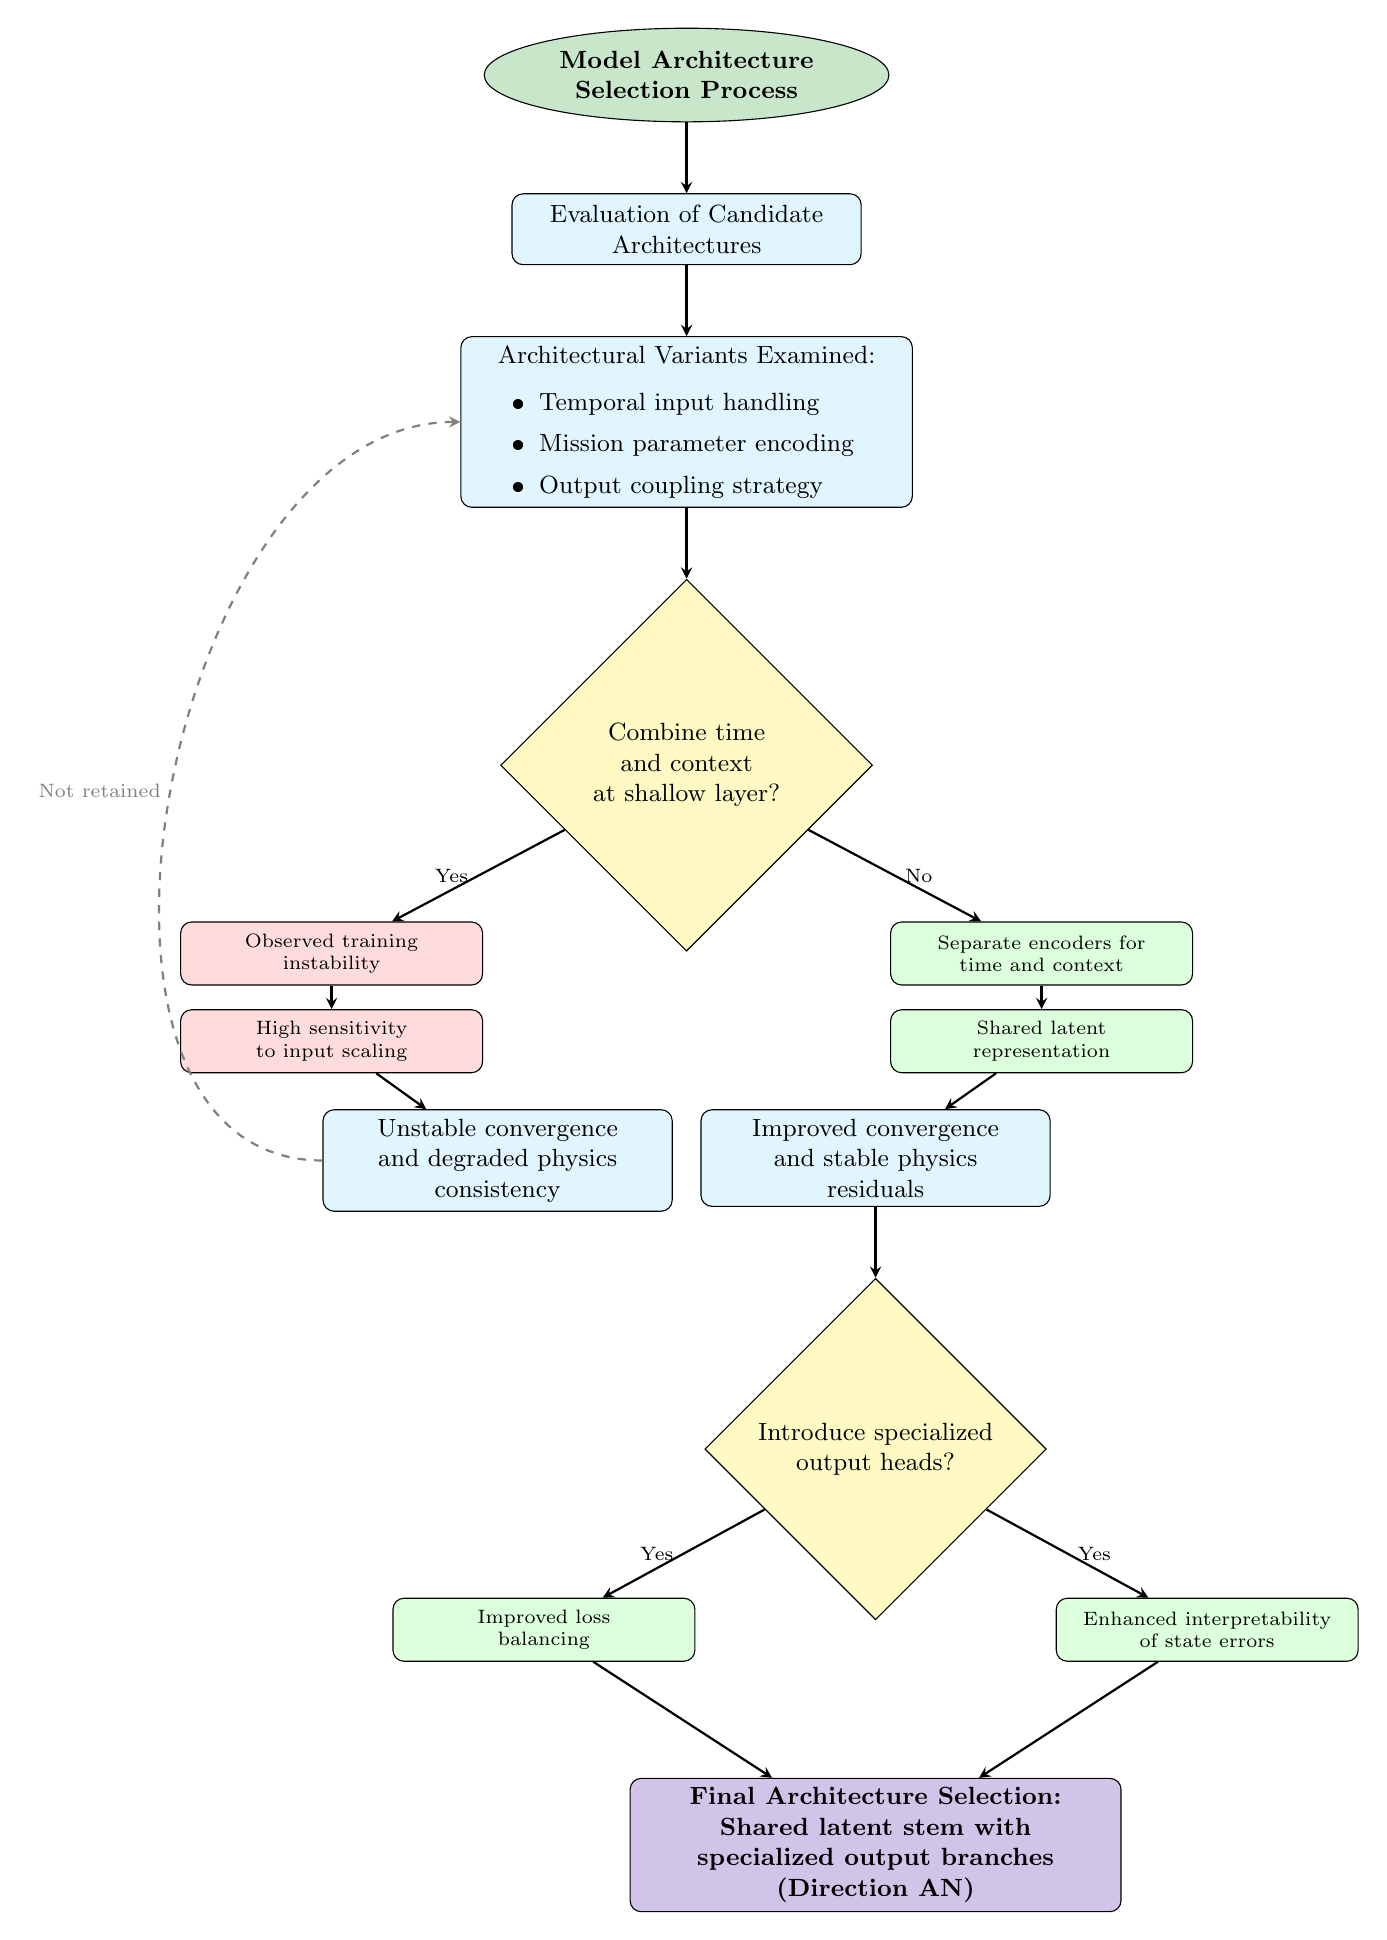
\begin{tikzpicture}[
    node distance=0.9cm and 1.6cm,
    every node/.style={font=\small},
    start/.style={
        ellipse, fill=startcolor, draw=black,
        text width=3.4cm, text centered,
        minimum height=0.9cm, font=\small\bfseries
    },
    process/.style={
        rectangle, rounded corners, fill=processcolor, draw=black,
        text width=4.2cm, text centered,
        minimum height=0.9cm
    },
    decision/.style={
        diamond, fill=decisioncolor, draw=black,
        text width=3.2cm, text centered,
        minimum height=1.1cm
    },
    issue/.style={
        rectangle, rounded corners, fill=issuecolor, draw=black,
        text width=3.6cm, text centered,
        minimum height=0.8cm, font=\scriptsize
    },
    good/.style={
        rectangle, rounded corners, fill=goodcolor, draw=black,
        text width=3.6cm, text centered,
        minimum height=0.8cm, font=\scriptsize
    },
    final/.style={
        rectangle, rounded corners, fill=finalcolor, draw=black,
        text width=4.6cm, text centered,
        minimum height=1.1cm, font=\small\bfseries
    },
    arrow/.style={->, >=stealth, thick}
]

% Start
\node[start] (start) {Model Architecture\\Selection Process};

% Evaluation
\node[process, below=of start] (evaluate) {Evaluation of Candidate\\Architectures};

\node[process, below=of evaluate, text width=5.5cm] (variants) {Architectural Variants Examined:\\
\begin{itemize}
\item Temporal input handling
\item Mission parameter encoding
\item Output coupling strategy
\end{itemize}
};

% Decision 1
\node[decision, below=of variants] (decision1) {Combine time and context\\at shallow layer?};

% Issue path
\node[issue, below left=0.8cm and 1.4cm of decision1] (issue1)
{Observed training\\instability};

\node[issue, below=0.3cm of issue1] (issue2)
{High sensitivity\\to input scaling};

% Good path
\node[good, below right=0.8cm and 1.4cm of decision1] (good1)
{Separate encoders for\\time and context};

\node[good, below=0.3cm of good1] (good2)
{Shared latent\\representation};

% Outcomes
\node[process, below=2.0cm of decision1, xshift=-2.4cm] (outcome1)
{Unstable convergence\\and degraded physics\\consistency};

\node[process, below=2.0cm of decision1, xshift=2.4cm] (outcome2)
{Improved convergence\\and stable physics\\residuals};

% Decision 2
\node[decision, below=of outcome2] (decision2)
{Introduce specialized\\output heads?};

% Benefits
\node[good, below left=0.8cm and 1.2cm of decision2] (benefit1)
{Improved loss\\balancing};

\node[good, below right=0.8cm and 1.2cm of decision2] (benefit2)
{Enhanced interpretability\\of state errors};

% Final
\node[final, below=2.0cm of decision2, text width=6cm] (final)
{Final Architecture Selection:\\
Shared latent stem with\\specialized output branches\\(Direction AN)};

% Arrows
\draw[arrow] (start) -- (evaluate);
\draw[arrow] (evaluate) -- (variants);
\draw[arrow] (variants) -- (decision1);

\draw[arrow] (decision1) -- node[left, font=\scriptsize] {Yes} (issue1);
\draw[arrow] (decision1) -- node[right, font=\scriptsize] {No} (good1);

\draw[arrow] (issue1) -- (issue2);
\draw[arrow] (issue2) -- (outcome1);

\draw[arrow] (good1) -- (good2);
\draw[arrow] (good2) -- (outcome2);

\draw[arrow] (outcome2) -- (decision2);

\draw[arrow] (decision2) -- node[left, font=\scriptsize] {Yes} (benefit1);
\draw[arrow] (decision2) -- node[right, font=\scriptsize] {Yes} (benefit2);

\draw[arrow] (benefit1) -- (final);
\draw[arrow] (benefit2) -- (final);

% Feedback loop
\draw[arrow, dashed, gray]
(outcome1.west) to[out=180, in=180]
node[left, font=\scriptsize] {Not retained}
(variants.west);

\end{tikzpicture}
\end{document}
